\documentclass[11pt,a4paper]{article}
\usepackage[margin=2.4cm]{geometry}
\usepackage{booktabs}
\usepackage{graphicx}
\usepackage{amsmath}
\usepackage[colorlinks=true,linkcolor=blue,urlcolor=blue]{hyperref}

\title{Solver hyperparameters for a hanging cable:\\
       Newton's defaults versus a tuned configuration}
\author{Generated by \texttt{analysis/sweep\_report.py}}
\date{\today}

\begin{document}
\maketitle

\section{What is being measured}

A cable of length $L = 0.893$~m hangs from
2 level supports spanning
$S = 0.350$~m, discretised into
60 segments and solved with Newton's
\texttt{add\_rod} plus the VBD solver.

Accuracy is the RMS distance from the \emph{analytic catenary} for the same
$L$ and $S$, not from another solver's answer. This matters: a configuration
cannot score well merely by agreeing with its neighbours, and the reference
costs no simulation time. The catenary assumes zero bending stiffness, which
for this cable is a very good approximation --- its $EI$ is small enough that
the analytic and simulated shapes agree to a millimetre --- so a deviation of
much more than that is numerical error rather than physics.

Two hyperparameters are swept, chosen because the configuration in this
repository differs sharply from every cable example shipped with Newton:

\begin{itemize}
  \item \textbf{Solver budget.} Newton's examples all use
        $\text{substeps} \times \text{iterations} = 10 \times 5 = 50$
        iteration-steps per frame. This repository uses $8 \times 200 = 1600$,
        a $32\times$ larger budget. The existing default was chosen by varying
        iterations alone at fixed substeps, so the substep axis was never
        tested.
  \item \textbf{Damping.} Newton's examples run
        $\text{bend\_damping}/\text{bend\_stiffness}$ between
        0.05 and 1.0. This repository's default sits
        at roughly $1.7\times10^{-3}$, between $30\times$ and $600\times$
        less damped.
\end{itemize}


\begin{figure}[htbp]
  \centering
  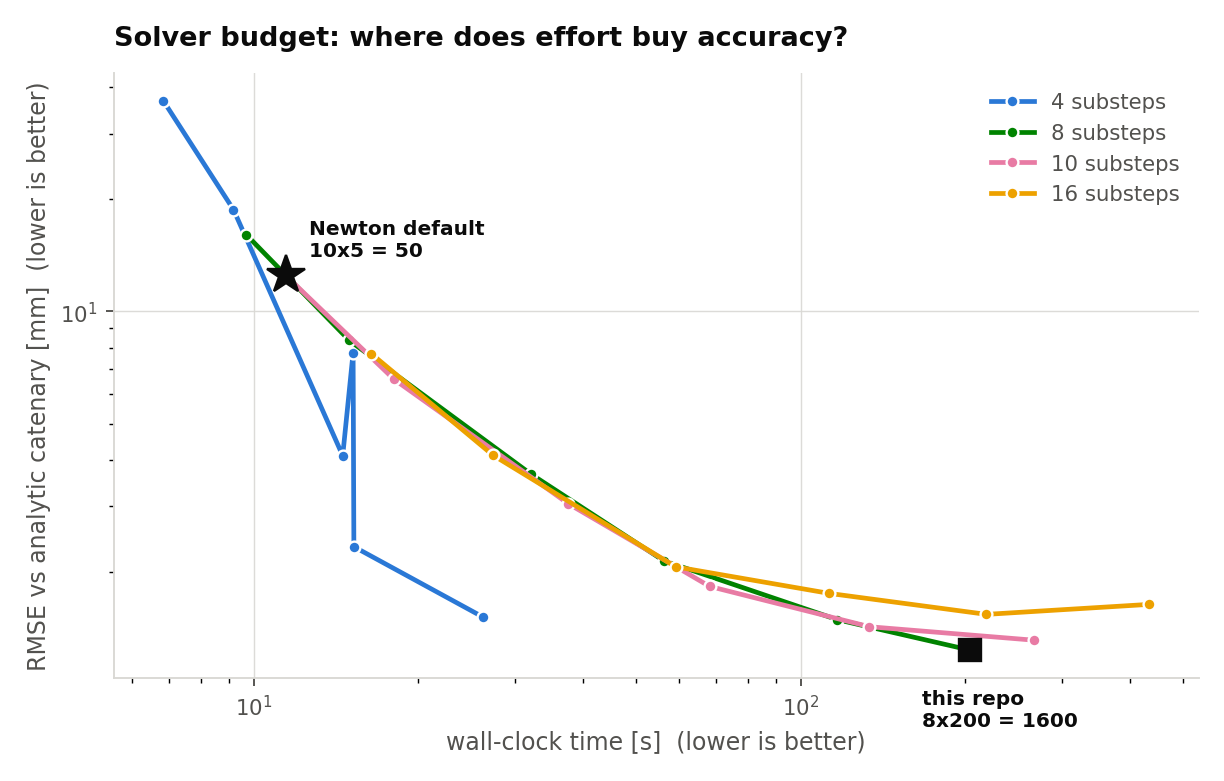
\includegraphics[width=\linewidth]{budget.png}
  \caption{Solver budget: accuracy against wall-clock cost. Both axes are logarithmic; the knee is where additional cost stops buying accuracy.}
\end{figure}

\begin{figure}[htbp]
  \centering
  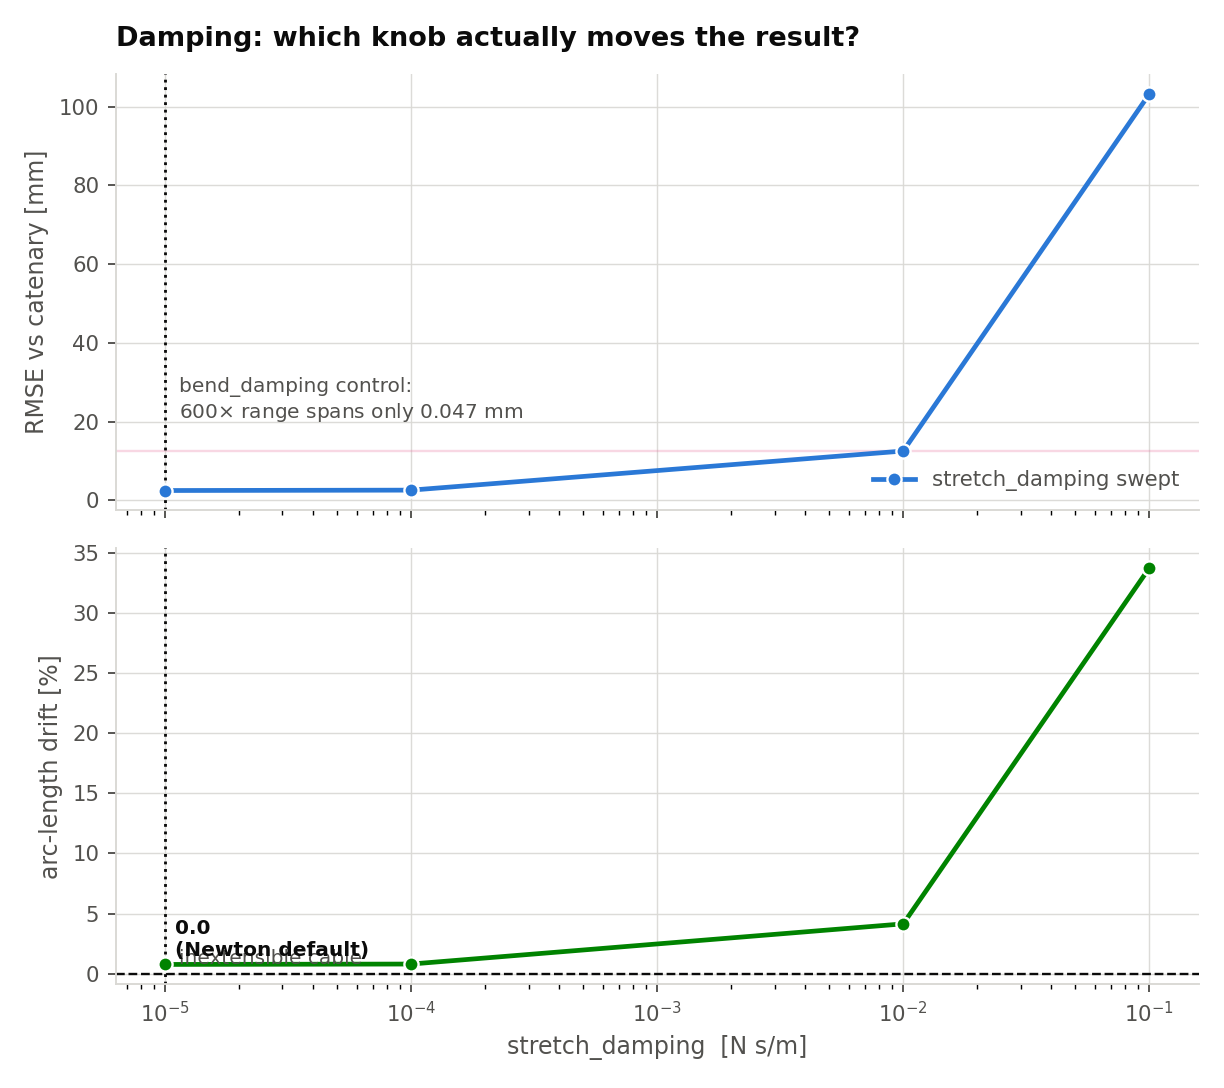
\includegraphics[width=\linewidth]{damping.png}
  \caption{Damping: accuracy and settling against the dimensionless damping ratio. The shaded band is the range spanned by Newton's own cable examples.}
\end{figure}


\section{Solver budget}

Newton's default reaches 12.50~mm RMSE in 11.4~s; this repository's default reaches 1.23~mm in 203.7~s, a 17.8$\times$ cost difference.

\begin{table}[htbp]
\centering
\small
\begin{tabular}{rrrrrrc}
\toprule
substeps & iterations & budget & RMSE [mm] & arc drift [\%] & wall [s] & settled \\
\midrule
    4 & 5 & 20 & 36.79 & +12.09 & 6.8 & no \\
    4 & 10 & 40 & 18.76 & +6.15 & 9.2 & no \\
    4 & 25 & 100 & 7.74 & +2.55 & 15.2 & yes \\
    4 & 50 & 200 & 4.10 & +1.34 & 14.5 & yes \\
    4 & 100 & 400 & 2.34 & +0.73 & 15.2 & yes \\
    4 & 200 & 800 & 1.51 & +0.43 & 26.2 & yes \\
    8 & 5 & 40 & 16.09 & +5.30 & 9.7 & no \\
    8 & 10 & 80 & 8.36 & +2.74 & 14.9 & no \\
    8 & 25 & 200 & 3.66 & +1.20 & 32.1 & no \\
    8 & 50 & 400 & 2.14 & +0.68 & 56.2 & no \\
    8 & 100 & 800 & 1.49 & +0.42 & 116.6 & no \\
    8 & 200 & 1600 & 1.23 & +0.29 & 203.7 & no \\
    10 & 5 & 50 & 12.50 & +4.14 & 11.4 & no \\
    10 & 10 & 100 & 6.58 & +2.16 & 18.0 & no \\
    10 & 25 & 250 & 3.04 & +0.97 & 37.6 & no \\
    10 & 50 & 500 & 1.83 & +0.57 & 68.1 & no \\
    10 & 100 & 1000 & 1.42 & +0.37 & 133.6 & no \\
    10 & 200 & 2000 & 1.31 & +0.27 & 267.3 & no \\
    16 & 5 & 80 & 7.70 & +2.53 & 16.4 & no \\
    16 & 10 & 160 & 4.11 & +1.36 & 27.4 & no \\
    16 & 25 & 400 & 2.06 & +0.65 & 59.1 & no \\
    16 & 50 & 800 & 1.75 & +0.41 & 112.6 & no \\
    16 & 100 & 1600 & 1.54 & +0.29 & 218.6 & no \\
    16 & 200 & 3200 & 1.64 & +0.23 & 433.9 & no \\
\bottomrule
\end{tabular}
\caption{Every budget configuration. ``budget'' is
substeps $\times$ iterations, the total iteration-steps per frame.}
\end{table}

\section{Damping}

Damping is reported as the dimensionless ratio
$\text{bend\_damping}/\text{bend\_stiffness}$, because the absolute
\texttt{bend\_damping} value is meaningless without the stiffness it damps ---
and the stiffness here is derived from beam theory ($EI/L_{\text{seg}}$),
not chosen to match Newton's demo numbers.

\begin{table}[htbp]
\centering
\small
\begin{tabular}{rrrrccr}
\toprule
bend\_damping & ratio & RMSE [mm] & arc drift [\%] & settled & $t_{\text{settle}}$ [s] & final $|v|_{\max}$ [m/s] \\
\midrule
    1.0e-04 & 0.001 & 12.50 & +4.14 & no & -- & 9.14e-03 \\
    1.0e-04 & 0.001 & 2.47 & +0.76 & yes & 4.70 & 1.66e-03 \\
    1.0e-04 & 0.001 & 2.56 & +0.79 & yes & 6.00 & 1.69e-03 \\
    1.0e-04 & 0.001 & 103.20 & +33.77 & yes & 4.40 & 1.82e-03 \\
    6.0e-02 & 0.888 & 12.55 & +4.14 & no & -- & 6.21e-03 \\
\bottomrule
\end{tabular}
\caption{Damping sweep at Newton's solver budget ($10\times5$), so the damping
effect is not confounded with a solver-effort effect.}
\end{table}

\section{How to read this}

\begin{itemize}
  \item \textbf{Arc drift is the check that needs no reference.} An
        inextensible cable must keep its length. Drift away from
        $0\%$ is the solver stretching the cable under its own weight, which is
        an artefact regardless of what the catenary says.
  \item \textbf{An unsettled run is provisional.} Where \emph{settled} is
        ``no'', the reported shape is a snapshot of a cable still in motion,
        averaged over the final window. Its RMSE is not comparable on equal
        terms with a settled run's, and this is exactly what the damping sweep
        is testing.
  \item \textbf{Cost is wall-clock on one machine.} Ratios between rows are
        meaningful; absolute seconds are not portable.
\end{itemize}

\end{document}
